%%% Simulering for design af snubber-kredsløb til MOSFET og diode %%%

\subsection{Snubber-kredsløb}
Figur~\ref{fig:simulering_diagram_snubber_3} viser det opdaterede diagram med snubber-kredsløbene indsat. Her ses det at primær-snubberen er placeret fra drain benet på MOSFET'en til ground, og sekundær-snubberen er placeret over dioden. 
\fxnote{Snubber skal placeres over MOSFET'en}
\begin{figure}[H]
	\center
	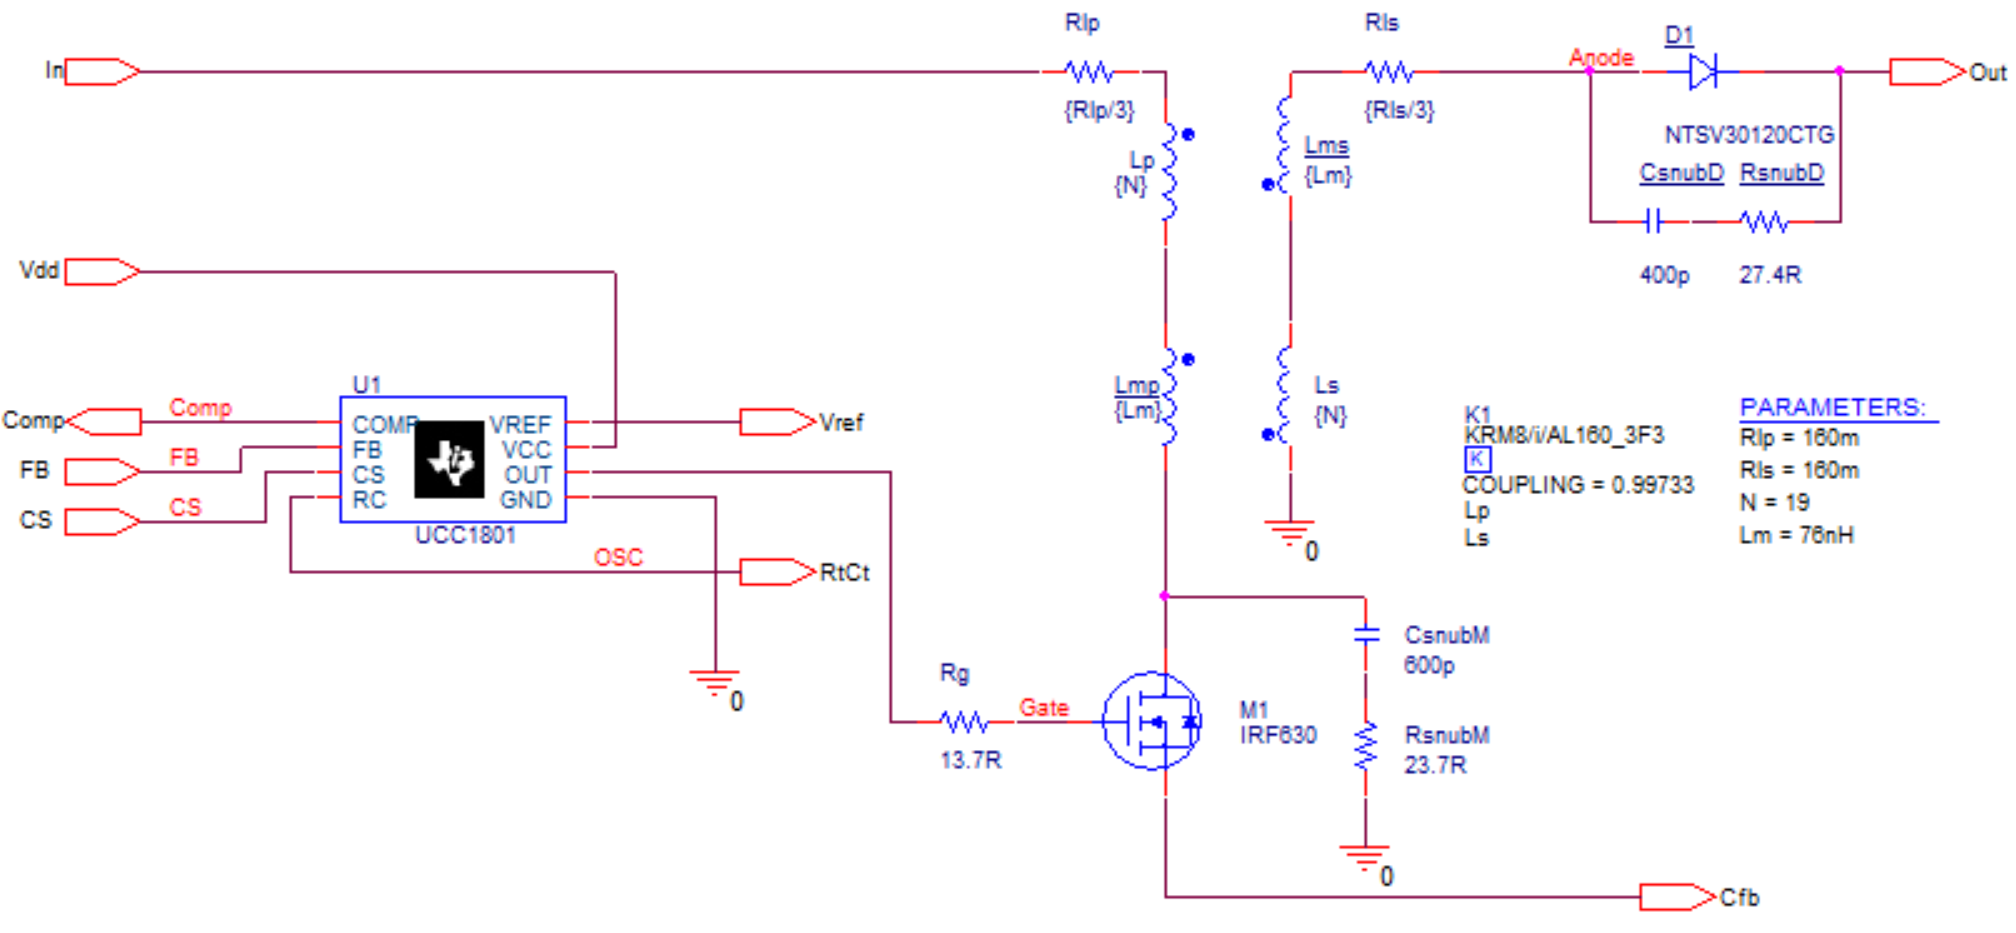
\includegraphics[max width=0.7\linewidth]{/tex/3iteration/billeder/Simulering/Simulering_power_diagram.PNG}
	\caption{Diagram for power modul med snubbere}
	\label{fig:simulering_diagram_snubber_3}
\end{figure}

\noindent Først måles MOSFET'ens drainspænding, i det tidspunk MOSFET'en går OFF, for at teste det primære snubber-kredsløb. Det er vist på figur~\ref{fig:simulering_snubber_MOSFET_3}. Her ses det, at svingningerne er blevet dæmpet ud, efter den første forventede svingning. Der kommer dog en lille anden svingning, som kommer da der er designet efter svingningerne aflæst i realiseringen, og ikke svingningerne aflæst i simuleringen for 2. iteration.  

\begin{figure}[H]
	\center
	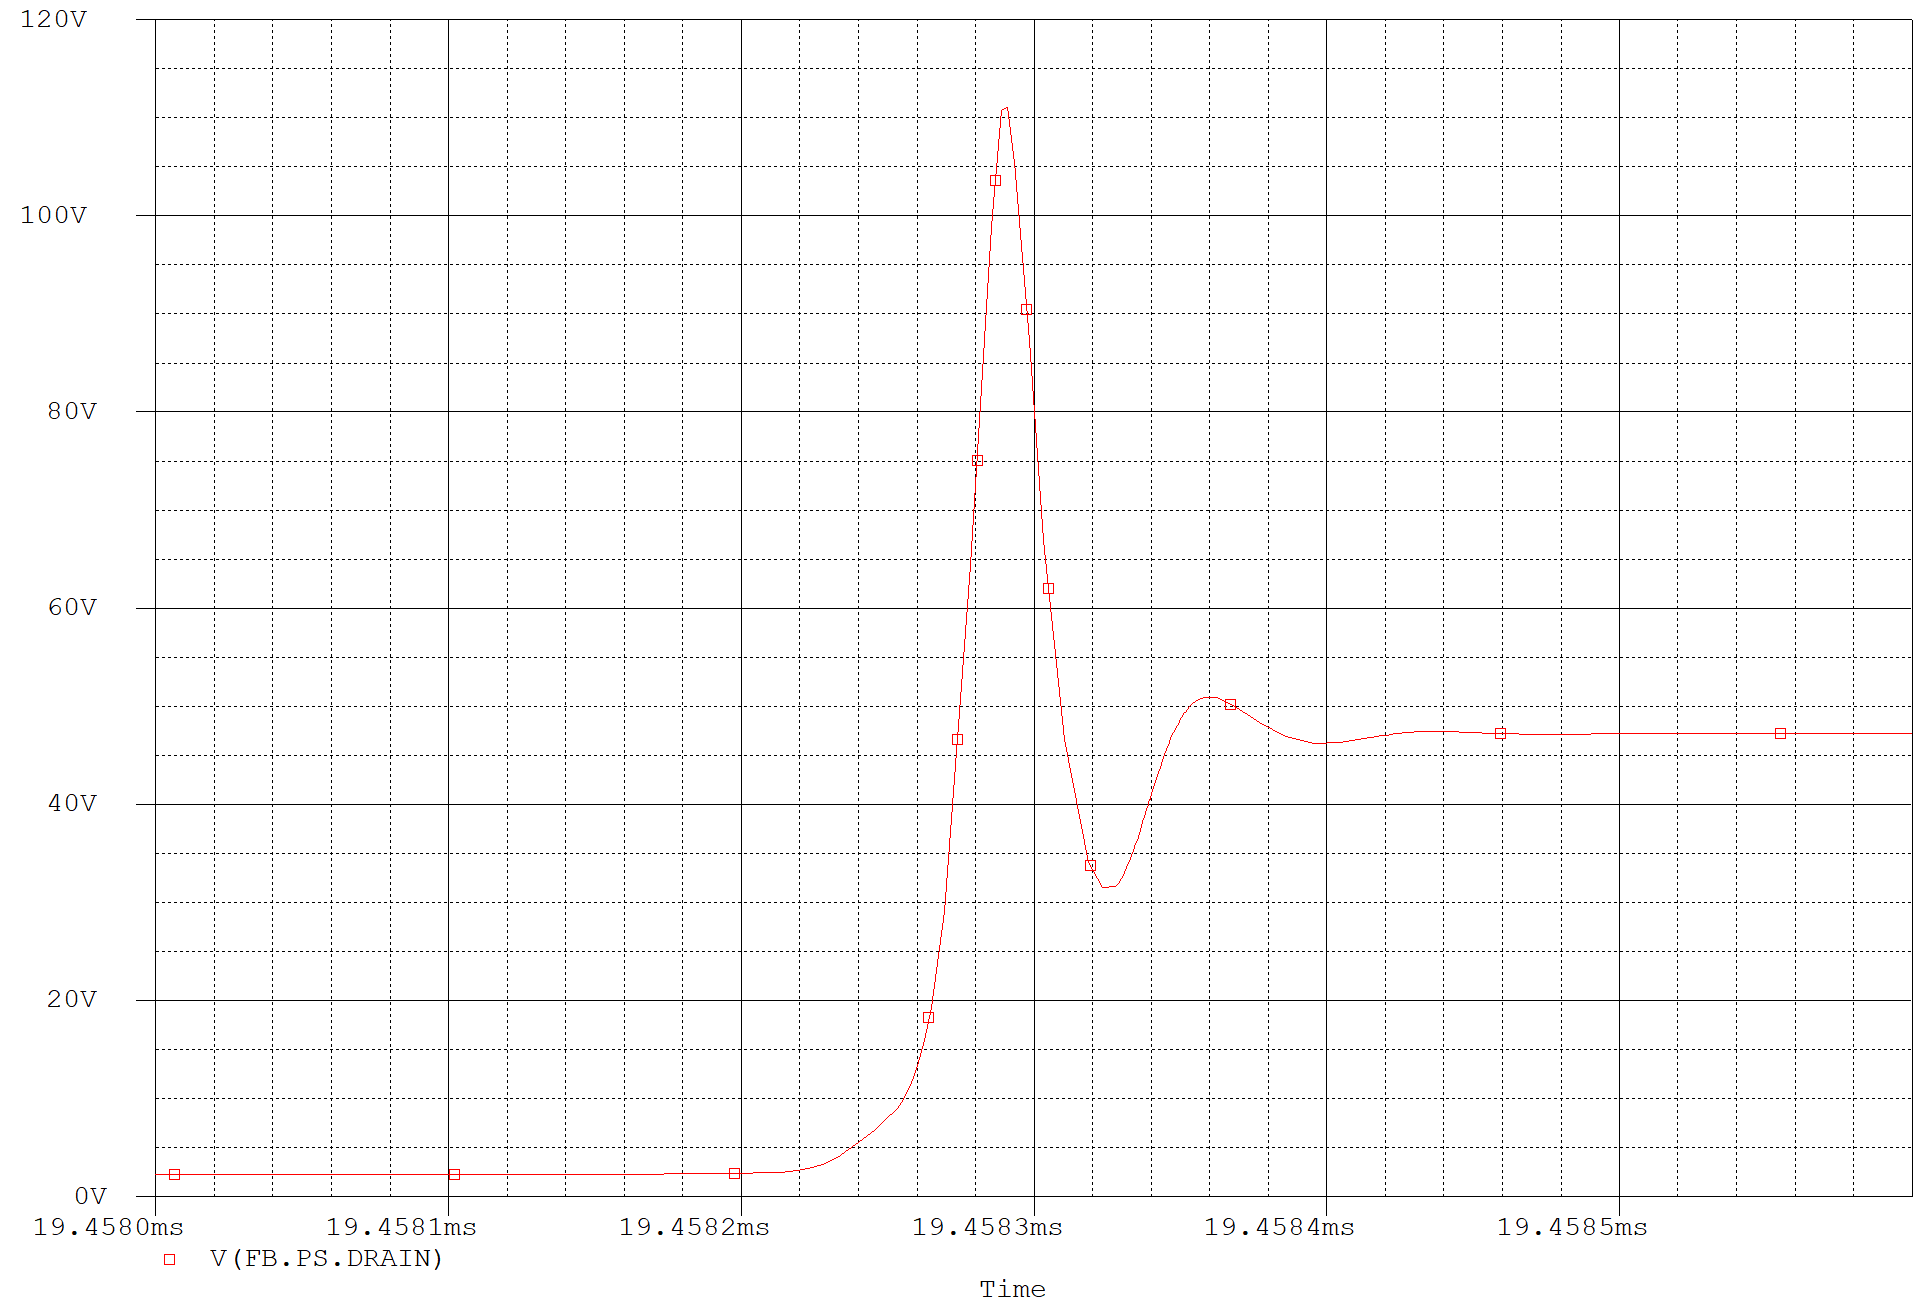
\includegraphics[max width=0.7\linewidth]{/tex/3iteration/billeder/Simulering/Simulering_snubber_MOSFET.PNG}
	\caption{Drain spænding efter snubber er tilføjet}
	\label{fig:simulering_snubber_MOSFET_3}
\end{figure}

\noindent Nu måles diodens anode spænding, i det tidspunkt MOSFET'en går ON, for at teste det sekundære snubber-kredsløb. Det er vist på figur~\ref{fig:simulering_snubber_diode_3}. Her ses det også, at snubber-kredsløbet har dæmpet de efterfølgende svingninger. Igen ses den lille anden svingning, da der er aflæst efter realiseringen.

\begin{figure}[H]
	\center
	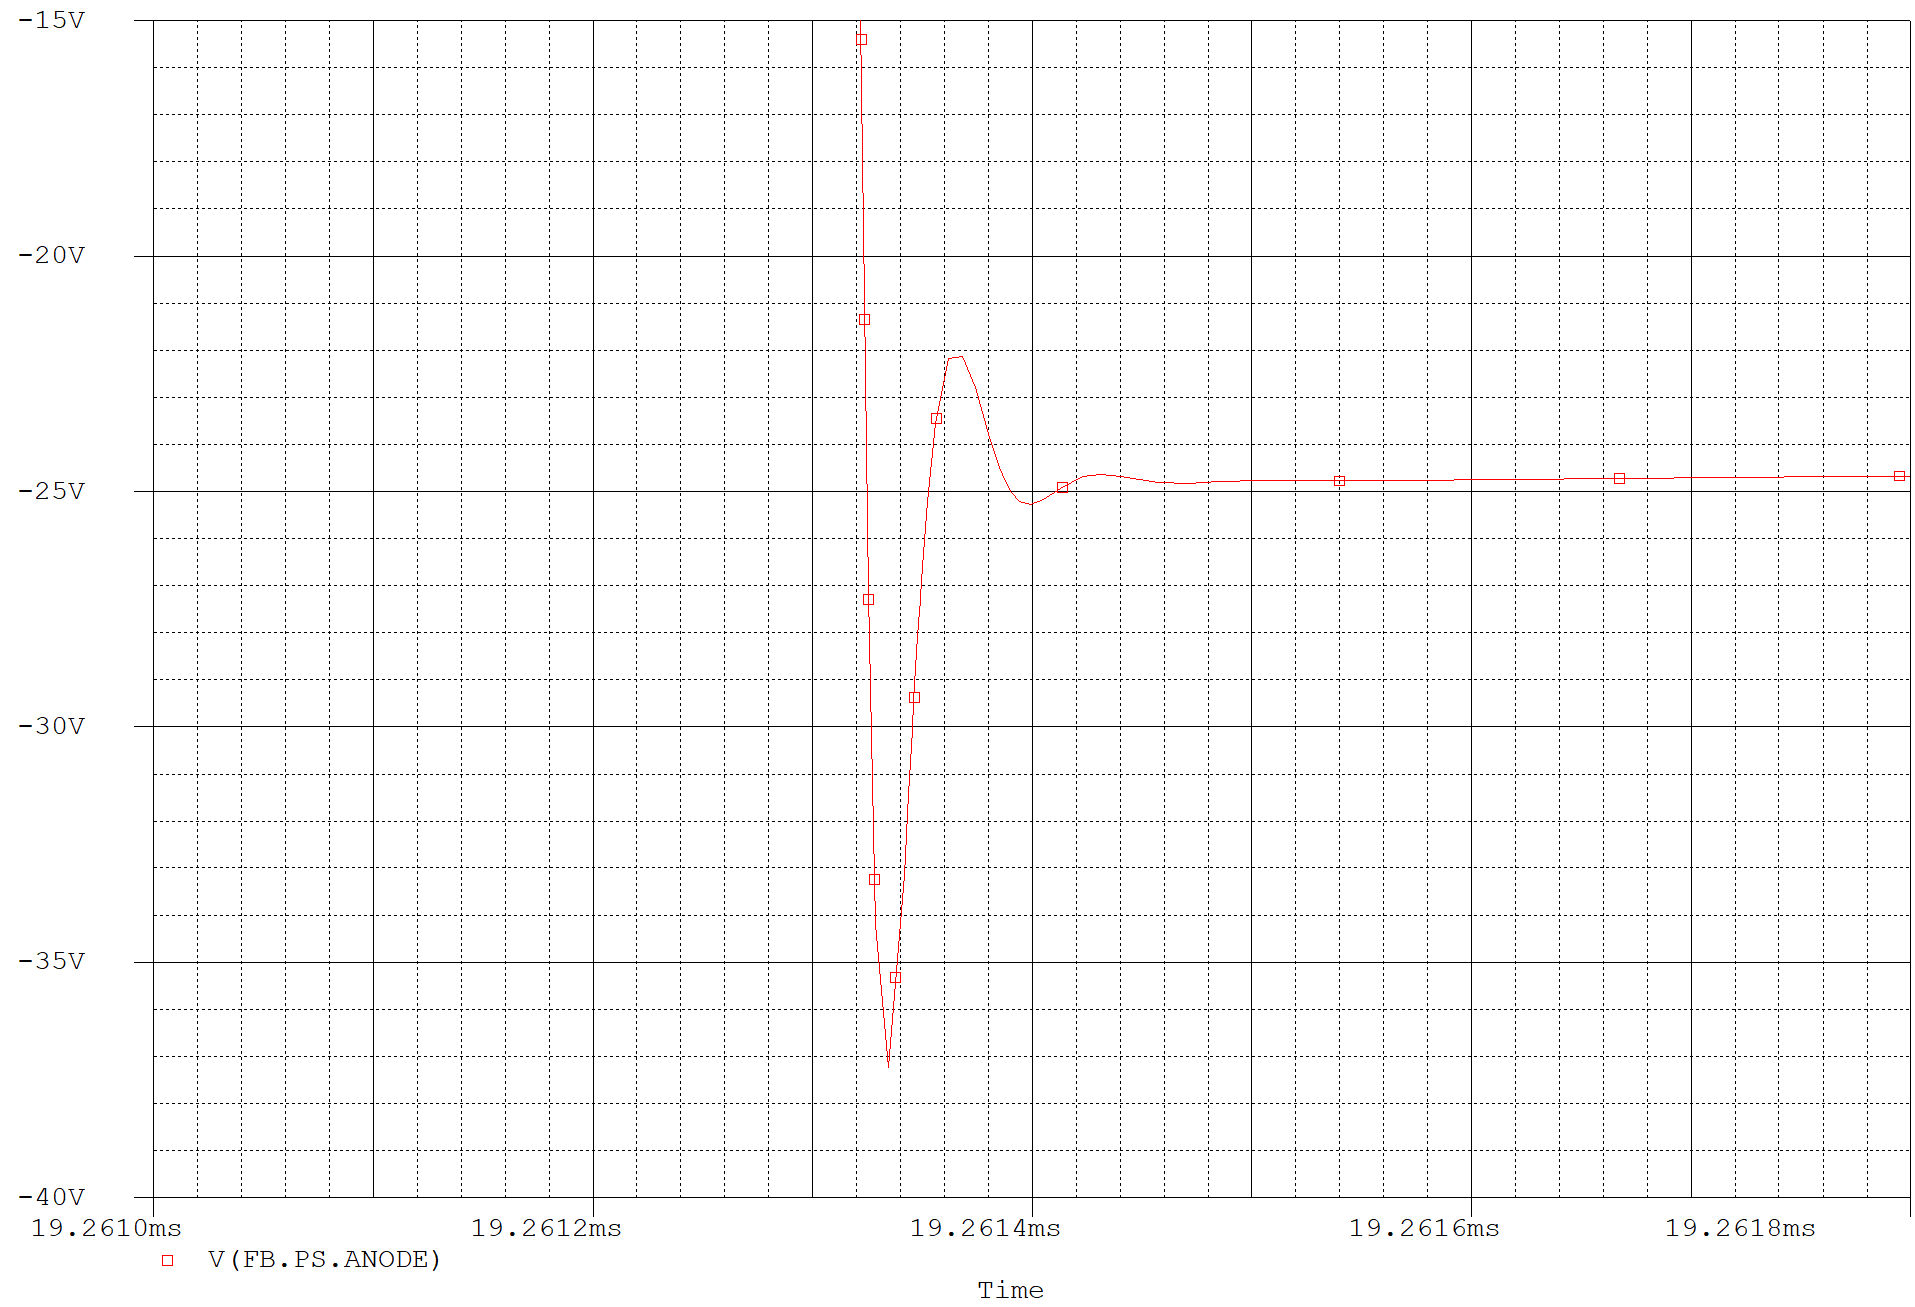
\includegraphics[max width=0.7\linewidth]{/tex/3iteration/billeder/Simulering/Simulering_snubber_diode.PNG}
	\caption{Anode spænding efter snubber er tilføjet}
	\label{fig:simulering_snubber_diode_3}
\end{figure}






